\section{Auswertung}
\begin{table}[H]
  \centering
   \begin{tabular}{c c c c c c}
    \toprule
    Material & Abmessungen [cm] & Dichte $ \rho\; [\frac{kg}{m^3}]$ & c $[\frac{J}{kgK}]$
    & $\kappa\; [\frac{W}{mK}]$ & $\Delta x$ [cm]\\
    \midrule
    Messing (breit) & 9*1,2*0,4 & 8520 & 385 & 120 & 3\\
    Messing (schmal) & 9*0,7*0,4 & 8520 & 385 & 120 & 3\\
    Aluminium       & 9*1,2*0,4 & 2800 & 830 & 237 & 3 \\
    Edelstahl       & 9*1,2*0,4 & 8000 & 400 & 15 & 3 \\

    \bottomrule
  \end{tabular}
  \caption{Gegebene Daten und Konstanten der verwendeten Metalle
  ($\kappa$ ist hier der nachgeschlagene Literaturwert)}
  \cite{skript}
  \cite{chemie}.
  \label{tab:daten}
\end{table}

\subsection{Statische Methode}
Zunächst werden die Messwerte T1 und T4 sowie T5 und T8 gegen die Zeit aufgetragen.
(Für die Bezeichnungen der Thermoelemente siehe Abbildung \ref{fig:aufbau})
\begin{figure}[H]
  \centering
  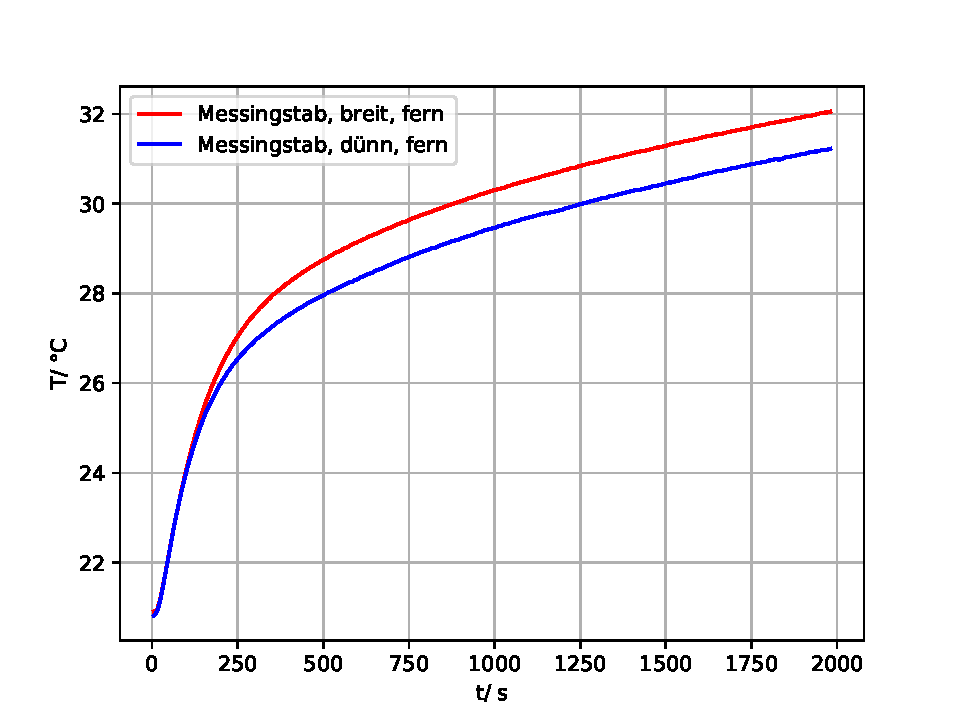
\includegraphics[height=7cm]{T14.pdf}
  \caption{Temperatur der Thermoelemente T1 und T4.}
  \label{fig:T14}
\end{figure}
\begin{figure}[H]
  \centering
  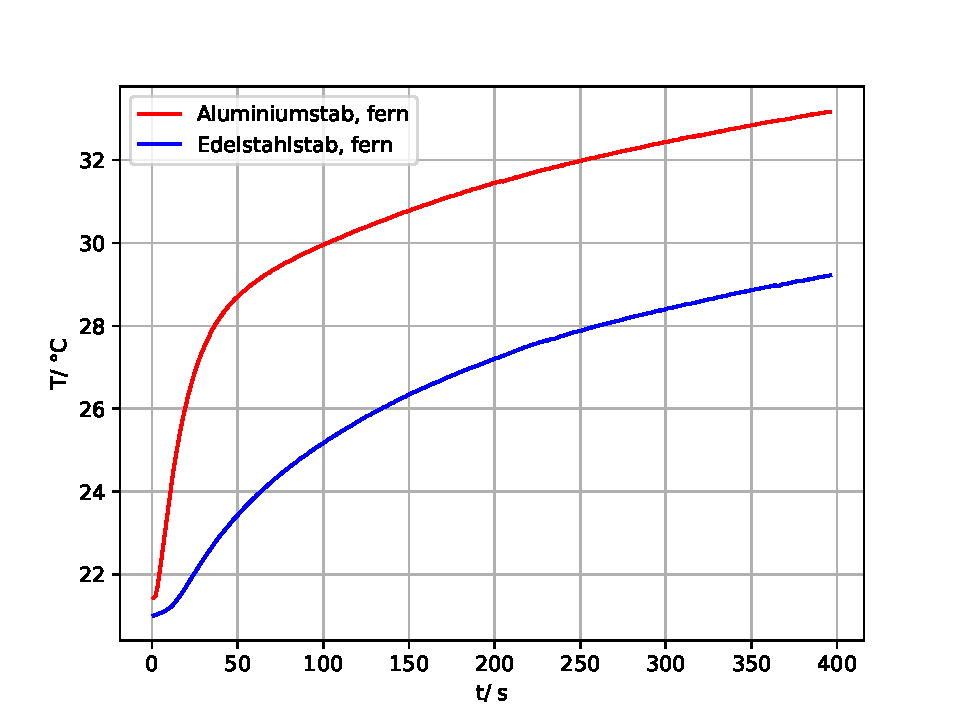
\includegraphics[height=7cm]{T58.pdf}
  \caption{Temperatur der Thermoelemente T5 und T8.}
  \label{fig:T58}
\end{figure}
Im Vergleich der Diagramme \ref{fig:T14} und \ref{fig:T58} fällt auf, dass
die Temperaturen exponentiel ansteigen. In Diagramm \ref{fig:T14} haben die
Stäbe zu Beginn die gleiche Temperatur, diese steigt circa bis zum Zeitpunkt
$t=\SI{150}{\s}$ sehr stark an. Danch flachen die Graphen ab und streben unterschiedliche
Temperaturen an. In Diagramm \ref{fig:T58} haben die Stäbe schon zu Beginn eine kleine
Temperaturdifferenz. Es ist deutlich zu erkennen, dass die Temperatur des
Aluminiumstabes viel schneller ansteigt, als die des Edelstahlstabes. Außerdem
strebt der Aluminiumstab während der gesamten Messung gegen eine höhere Temperatur.\\
Im folgenden werden die Temperaturen zum Zeitpunkt $t=\SI{700}{\s}$ notiert:

\begin{align*}
  T1 &=\SI{29,48}{\celsius}\\
  T4 &=\SI{28,65}{\celsius}\\
  T5 &=\SI{29,48}{\celsius}\\
  T8 &=\SI{26,13}{\celsius}.
\end{align*}

Aus den Diagrammen \ref{fig:T14} und \ref{fig:T58}, als auch aus den notierten
Temperaturen kann abgelesen werden, dass T5 (Aluminiumstab) die höchste Temperatur erreicht.
Daraus kann gefolgert werden, dass Aluminium die Wärme am besten leitet. Am schlechtesten
leitet Edelstahl die Wärme. Das der breite Messingstab die Wärme besser leitet als der
dünne Messingstab dann dadurch begründet werden, dass $\kappa \propto A$ gilt und
der dünne Messingstab deshalb eine geringere Wärmeleitfähigkeut besitzt.\\

Im Folgenden wird der Wärmestrom $\frac{\Delta Q}{\Delta t}$
der Metalle nach der Formel \ref{eqn:warm} berechnet.
Die Werte der Wärmeleitfähigkeit $\kappa$ wurden aus der Literatur \cite{chemie} entnommen.
Der Abstand $\Delta x$ zwischen den Thermoelenten wurde gemessen, die restlichen
Werte wurden aus der Versuchsanleitung \cite{skript} entnommen.
\begin{table}[H]
  \centering
   \begin{tabular}{c c c c c}
    \toprule
     Zeit t/\;s & $(T_{2}-T{1})$/\;K & $\frac{\Delta Q_{12}}{\Delta t}$ /\;W &
     $(T_{7}-T_{8})$/\;K & $\frac{\Delta Q_{78}}{\Delta t}$ /\;W \\
    \midrule
    100 & 1,95 & -0,37 & 4,06 & -0,09 \\
    200 & 1,30 & -0,25  & 4,24 & -0,10 \\
    300 & 0,97 & -0,19 & 3,96 & -0,09 \\
    400 & 0,82 & -0,16  & 3,72 & -0,08\\
    500 & 0,75 & -0,14  &  3,55 & -0,09\\

    \bottomrule
  \end{tabular}
  \caption{Temperaturdifferenzen $(T_{2}-T_{1})$ und $(T_{7}-T{8})$ mit zugehörigem
  Wärmestrom.}
  \label{tab:tab1}
\end{table}

\begin{table}[H]
  \centering
   \begin{tabular}{c c c c c}
    \toprule
     Zeit t/\;s & $(T_{3}-T{4})$/\;K & $\frac{\Delta Q_{34}}{\Delta t}$ /\;W &
     $(T_{6}-T_{5})$/\;K & $\frac{\Delta Q_{56}}{\Delta t}$ /\;W \\
    \midrule
    100 & 2,37 & -0,46 & 1,26 & -0,48 \\
    200 & 1,72 & -0,33  & 0,79 & -0,29 \\
    300 & 1,43 & -0,27 & 0,61 & -0,23 \\
    400 & 1,31 & -0,25  & 0,55 & -0,21\\
    500 & 1,25 & -0,24  &  0,52 & -0,19\\

    \bottomrule
  \end{tabular}
  \caption{Temperaturdifferenzen $(T_{3}-T_{4})$ und $(T_{6}-T{5})$ mit zugehörigem
  Wärmestrom.}
  \label{tab:tab1}
\end{table}

Die Ergebnisse für den Wärmestrom werden nach
\begin{equation}
  \bar{x}=\frac{1}{N}\sum_{1}^N x_{i}
  \label{eqn:mittel}
\end{equation}
gemittelt und der zugehörige Fehler berechnet sich nach
\begin{equation}
  \Delta\bar x = \frac{1}{N}\sqrt{\frac{1}{N-1}\cdot\sum_{1}^N (x_{i}-\bar x)^2}.
  \label{eqn:gauß}
\end{equation}
Somit ergeben sich folgende Werte:
\begin{align*}
  \frac{\Delta Q_{12}}{\Delta t} &=\SI{-0,22(04)}{\W}\;\;\;    &\frac{\Delta Q_{34}}{\Delta t} &=\SI{-0,28(04)}{\W}\\
  \frac{\Delta Q_{56}}{\Delta t} &=\SI{-0,31(03)}{\W}\;\;\;    &\frac{\Delta Q_{78}}{\Delta t} &=\SI{-0,09(00)}{\W}
\end{align*}

Da $\frac{\Delta Q}{\Delta t}$ proportional zu $\kappa$ und der Querschnittsfläche $A$ ist,
ist zu erwartem, dass der Wärmestrom von Aluminium an größten ist. Das wird auch durch die Messwerte bestätigt.
Edelstahl sollte von den vorliegenden Metallen den gringsten Wärmestrom aufweisen, doch das wird
nicht durch die Messung  bestätigt. Es ist aber deutlich zu erkennen, dass der Wärmestrom des breiten
Messingstabes größer ist, als der des schmalen Messingstabes. Dieses Ergebnis war aufgrund von
$\frac{\Delta Q}{\Delta t} \propto \kappa$ zu erwarten.
Das Minuszeichen lässt sich dadurch erklären, das die Wärme immer vom wärmeren zum
kältereen Wärmereservoir fließt.
\\
In Diagramm \ref{fig:diff} sind die Temperaturdifferenzen $T_{7}-T_{8}$ und $T_{2}-T_{1}$
dargestellt. Auffällig ist, das beide Graphen zu Beginn sehr stark ansteigen und ein
Maximum erreichen. Anschließend fallen beide Graphen ab und verlaufen dann parallel zu t-Achse.
Insgesamt liegt der Graph des Edelstahlstabes $\Delta T_{78}$ deutlich über dem des breiten
Messingstabes $\Delta T_{21}$.
\begin{figure}[H]
  \centering
  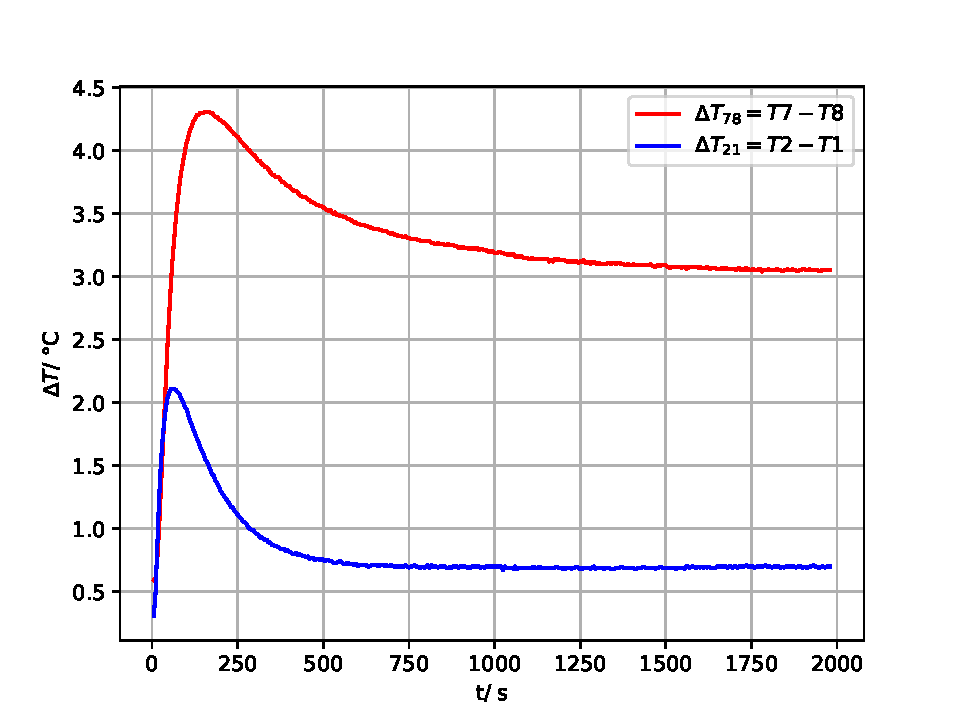
\includegraphics[height=7cm]{T7821.pdf}
  \caption{Temperaturdifferenz $T_{7}-T_{8}$ und $T_{2}-T_{1}$ aufgetragen gegen die Zeit.}
  \label{fig:diff}
\end{figure}

\subsection{Dynamische Methode}
In diesem Teil wird die Wärmeleitfähigkeit $\kappa$ der verschiedenen Materialien bestimmt.
Die Messwerte der verschiedenen Materialien werden graphisch in
den Dagrammen \ref{fig:T12}, \ref{fig:T56} und \ref{fig:T78} dargestellt. Daraus
werden die Werte für die Amplitude und die Phasendifferenz $\Delta x$ abgelesen.

Im Folgenden sind die Temperaturverläufe der verschiedenen Metalle sowie die abgelesen
Daten dargestellt.
\begin{figure}[H]
  \centering
  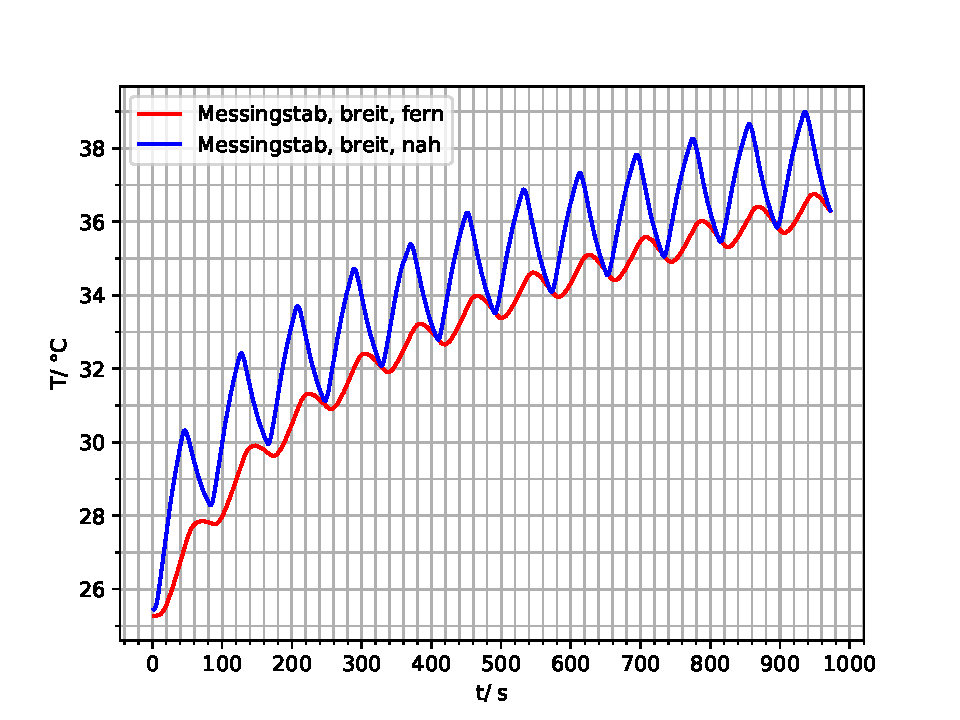
\includegraphics[height=8cm]{T12.pdf}
  \caption{Temperaturverlauf des breiten Messingstabes, Periodendauer 80s.}
  \label{fig:T12}
\end{figure}
\begin{figure}[H]
  \centering
  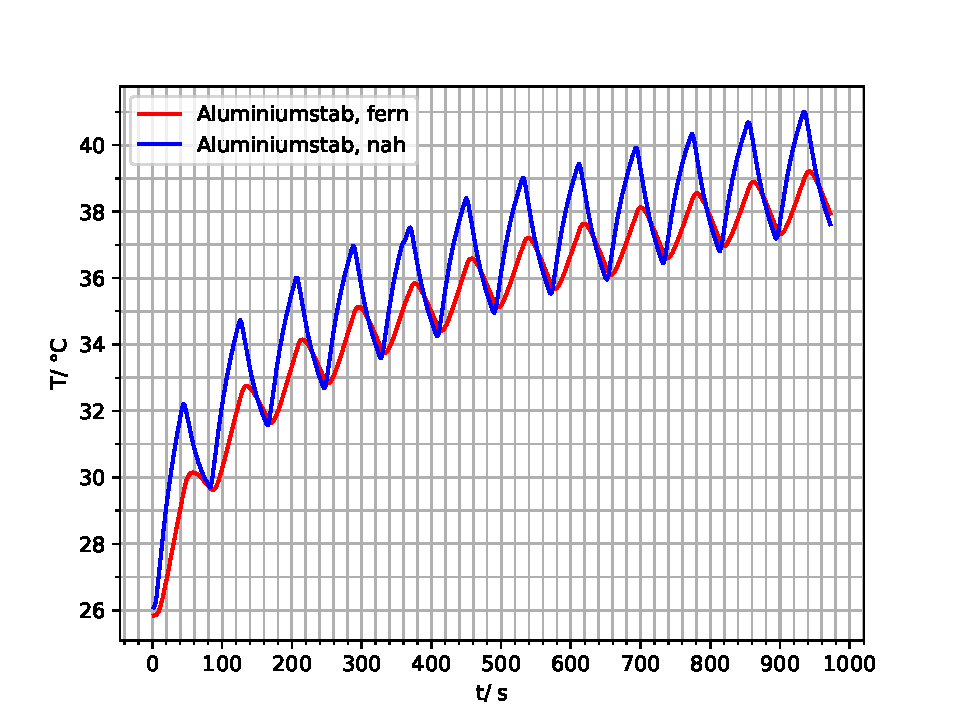
\includegraphics[height=8cm]{T56.pdf}
  \caption{Temperaturverlauf des Aluminiumstabes, Periodendauer 80s.}
  \label{fig:T56}
\end{figure}
\begin{figure}[H]
  \centering
  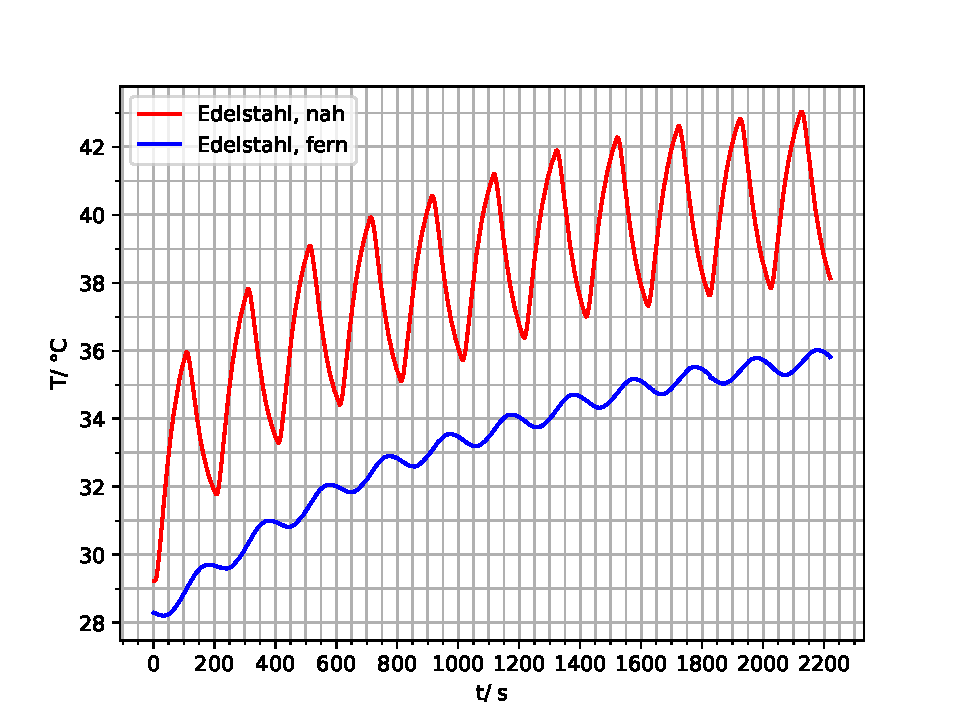
\includegraphics[height=8cm]{T78.pdf}
  \caption{Temperaturverlauf des Edelstahlstabes,Periodendauer 200s.}
  \label{fig:T78}
\end{figure}

\begin{table}[H]
  \centering
   \begin{tabular}{c c c c}
    \toprule
     $A_{nah}$/ K & $A_{fern}$/ K & $\ln{\frac{A_{nah}}{A_{fern}}}$/ K & Phasendifferenz $\Delta t$/ s\\
    \midrule
    3,2 & 1,0 & 1,16 & 10 \\
    3,2 & 1,2 & 0,98 & 18 \\
    3,3 & 1,1 & 1,10 & 19 \\
    3,1 & 1,1 & 1,04 & 19 \\
    3,1 & 1,0 & 1,13 & 16 \\
    2,9 & 1,0 & 1,06 & 12 \\
    3,0 & 0,8 & 1,32 & 10 \\
    3,0 & 0,9 & 1,20 & 12 \\
    3,0 & 0,8 & 1,32 & 11 \\
    3,0 & 0,9 & 1,20 & 11 \\
    2,9 & 0,8 & 1,28 & 11 \\

    \bottomrule
  \end{tabular}
  \caption{Amplituden und Phasenverschiebung des Messingstabes.}
  \label{tab:tab2}
\end{table}

\begin{table}[H]
  \centering
   \begin{tabular}{c c c c}
    \toprule
     $A_{nah}$/ K & $A_{fern}$/ K & $\ln{\frac{A_{nah}}{A_{fern}}}$/ K & Phasendifferenz $\Delta t$/ s\\
    \midrule
    4,1 & 2,1 & 0,67 & 6\\
    3,9 & 2,1 & 0,62 & 4\\
    3,9 & 1,9 & 0,72 & 6\\
    3,8 & 1,8 & 0,75 & 6\\
    3,6 & 1,9 & 0,64 & 6\\
    4,0 & 1,8 & 0,79 & 8\\
    3,8 & 1,5 & 0,93 & 6\\
    3,6 & 1,9 & 0,64 & 6\\
    3,9 & 1,9 & 0,72 & 6\\
    3,7 & 1,9 & 0,67 & 4\\
    3,7 & 1,9 & 0,67 & 2\\
    3,8 & 1,5 & 0,93 & 4\\
    \bottomrule
  \end{tabular}
  \caption{Amplituden und Phasenverschiebung des Aluminiumstabes.}
  \label{tab:tab3}
\end{table}

\begin{table}[H]
  \centering
   \begin{tabular}{c c c c}
    \toprule
     $A_{nah}$/ K & $A_{fern}$/ K & $\ln{\frac{A_{nah}}{A_{fern}}}$/ K & Phasendifferenz $\Delta t$/ s\\
    \midrule
    5,5 & 0,8 & 1,93 & 50 \\
    5,4 & 0,7 & 2,04 & 48 \\
    5,2 & 0,6 & 2,16 & 48 \\
    5,0 & 0,7 & 1,97 & 49 \\
    5,0 & 0,6 & 2,12 & 48 \\
    5,1 & 0,6 & 2,14 & 50 \\
    5,2 & 0,7 & 2,01 & 48 \\
    5,1 & 0,6 & 2,14 & 48 \\
    5,1 & 0,7 & 1,98 & 48 \\
    5,0 & 0,6 & 2,12 & 49\\
    \bottomrule
  \end{tabular}
  \caption{Amplituden und Phasenverschiebung des Edelstahlstabes.}
  \label{tab:tab4}
\end{table}


Mit Gleichung \ref{eqn:mittel} und \ref{eqn:gauß} ergeben sich aus den Tabellen
\ref{tab:tab2}, \ref{tab:tab3} und \ref{tab:tab4} folgende Werte:
\begin{align*}
  \text{Messingstab}: \ln{\frac{A_{nah}}{A_{fern}}} &=\SI{1,16(10)}\;\;\; &\Delta t &=\SI{13,54(38)}{\s}  \\
  \text{Aluminiumstab}: \ln{\frac{A_{nah}}{A_{fern}}} &=\SI{0,73(00)}\;\;\; &\Delta t &=\SI{4,84(22)}{\s}   \\
  \text{Edelstahlstab}: \ln{\frac{A_{nah}}{A_{fern}}} &=\SI{2,07(00)}\;\;\; &\Delta t &=\SI{48,60(08)}{\s}
\end{align*}

Aus diesen Werten und den Angaben aus Tabelle \ref{tab:tab1} lässt sich mit Hilfe der Formel \ref{eqn:leitf}
die Wärmeleitfähigkeit $\kappa$ bestimmen:
\begin{align*}
  \kappa_{Messing} &=\SI{93,98(1074)}{\W\per\meter\kelvin} \\
  \kappa_{Aluminium} &=\SI{295,99(1345)}{\W\per\meter\kelvin} \\
  \kappa_{Edelstahl} &=\SI{14,31(02)}{\W\per\meter\kelvin}
\end{align*}

\label{sec:Auswertung}


%\begin{figure}
%  \centering
%  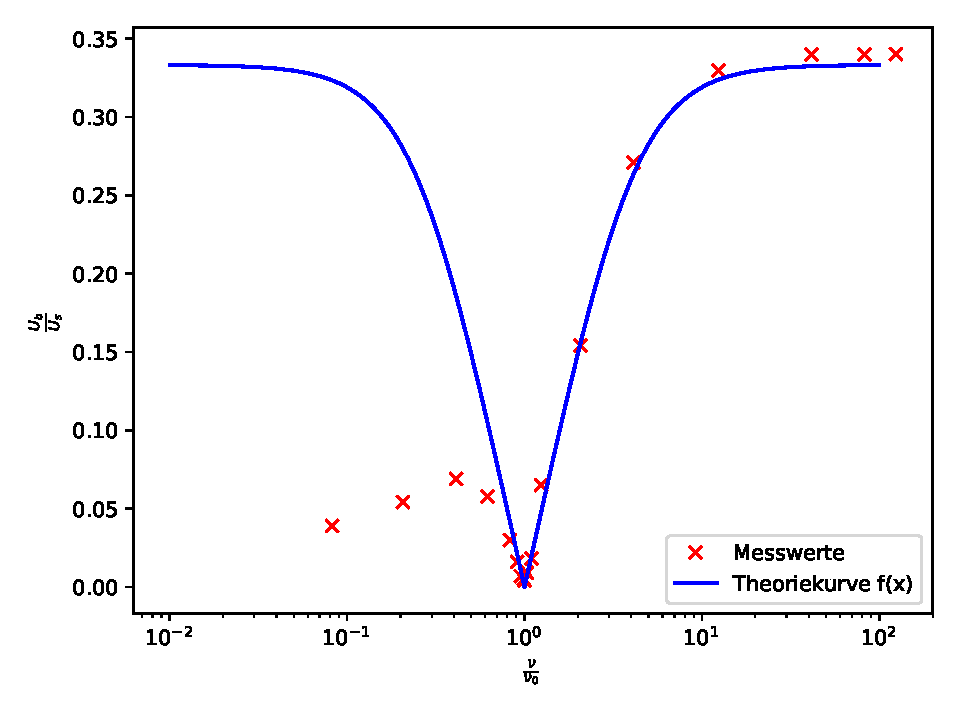
\includegraphics{plot.pdf}
%  \caption{Plot.}
%  \label{fig:plot}
%\end{figure}
